%package list
\documentclass{article}
\usepackage[top=3cm, bottom=3cm, outer=3cm, inner=3cm]{geometry}
\usepackage{multicol}
\usepackage{graphicx}
\usepackage{url}
%\usepackage{cite}
\usepackage{hyperref}
\usepackage{array}
%\usepackage{multicol}
\newcolumntype{x}[1]{>{\centering\arraybackslash\hspace{0pt}}p{#1}}
\usepackage{natbib}
\usepackage{pdfpages}
\usepackage{multirow}
\usepackage[normalem]{ulem}
\useunder{\uline}{\ul}{}
\usepackage{svg}
\usepackage{xcolor}
\usepackage{listings}
\lstdefinestyle{ascii-tree}{
    literate={├}{|}1 {─}{--}1 {└}{+}1 
  }
\lstset{basicstyle=\ttfamily,
  showstringspaces=false,
  commentstyle=\color{red},
  keywordstyle=\color{blue}
}
%\usepackage{booktabs}
\usepackage[labelformat=empty]{caption}
\usepackage{subcaption}
\usepackage{float}
\usepackage{array}

\newcolumntype{M}[1]{>{\centering\arraybackslash}m{#1}}
\newcolumntype{N}{@{}m{0pt}@{}}


%%%%%%%%%%%%%%%%%%%%%%%%%%%%%%%%%%%%%%%%%%%%%%%%%%%%%%%%%%%%%%%%%%%%%%%%%%%%
%%%%%%%%%%%%%%%%%%%%%%%%%%%%%%%%%%%%%%%%%%%%%%%%%%%%%%%%%%%%%%%%%%%%%%%%%%%%
\newcommand{\itemEmail}{cmestasz@unsa.edu.pe}
\newcommand{\itemStudent}{Christian Mestas Zegarra}
\newcommand{\itemCourse}{Fundamentos de la Programación 2}
\newcommand{\itemCourseCode}{1701213}
\newcommand{\itemSemester}{II}
\newcommand{\itemUniversity}{Universidad Nacional de San Agustín de Arequipa}
\newcommand{\itemFaculty}{Facultad de Ingeniería de Producción y Servicios}
\newcommand{\itemDepartment}{Departamento Académico de Ingeniería de Sistemas e Informática}
\newcommand{\itemSchool}{Escuela Profesional de Ingeniería de Sistemas}
\newcommand{\itemAcademic}{2023 - B}
\newcommand{\itemInput}{Del 15 Enero 2024}
\newcommand{\itemOutput}{Al 22 Enero 2024}
\newcommand{\itemPracticeNumber}{22}
\newcommand{\itemTheme}{Interfaz Gráfica de Usuario}
%%%%%%%%%%%%%%%%%%%%%%%%%%%%%%%%%%%%%%%%%%%%%%%%%%%%%%%%%%%%%%%%%%%%%%%%%%%%
%%%%%%%%%%%%%%%%%%%%%%%%%%%%%%%%%%%%%%%%%%%%%%%%%%%%%%%%%%%%%%%%%%%%%%%%%%%%

\usepackage[english,spanish]{babel}
\usepackage[utf8]{inputenc}
\AtBeginDocument{\selectlanguage{spanish}}
\renewcommand{\figurename}{Figura}
\renewcommand{\refname}{Referencias}
\renewcommand{\tablename}{Tabla} %esto no funciona cuando se usa babel
\AtBeginDocument{%
	\renewcommand\tablename{Tabla}
}

\usepackage{fancyhdr}
\pagestyle{fancy}
\fancyhf{}
\setlength{\headheight}{30pt}
\renewcommand{\headrulewidth}{1pt}
\renewcommand{\footrulewidth}{1pt}
\fancyhead[L]{\raisebox{-0.2\height}{
\includegraphics[width=3cm]{img/logo_episunsa.png}}}
\fancyhead[C]{\fontsize{7}{7}\selectfont	\itemUniversity \\ \itemFaculty \\ \itemDepartment \\ \itemSchool \\ \textbf{\itemCourse}}
\fancyhead[R]{\raisebox{-0.2\height}{
\includegraphics[width=1.2cm]{img/logo_abet}}}
\fancyfoot[L]{Christian Mestas}
\fancyfoot[C]{\itemCourse}
\fancyfoot[R]{Página \thepage}

% para el codigo fuente
\usepackage{listings}
\usepackage{color, colortbl}
\definecolor{dkgreen}{rgb}{0,0.6,0}
\definecolor{gray}{rgb}{0.5,0.5,0.5}
\definecolor{mauve}{rgb}{0.58,0,0.82}
\definecolor{codebackground}{rgb}{0.95, 0.95, 0.92}
\definecolor{tablebackground}{rgb}{0.8, 0, 0}

\lstset{frame=tb,
	language=bash,
	aboveskip=3mm,
	belowskip=3mm,
	showstringspaces=false,
	columns=flexible,
	basicstyle={\small\ttfamily},
	numbers=none,
	numberstyle=\tiny\color{gray},
	keywordstyle=\color{blue},
	commentstyle=\color{dkgreen},
	stringstyle=\color{mauve},
	breaklines=true,
	breakatwhitespace=true,
	tabsize=3,
	backgroundcolor= \color{codebackground},
}

\begin{document}

\vspace*{10px}

\begin{center}
	\fontsize{17}{17} \textbf{ Informe de Laboratorio \itemPracticeNumber}
\end{center}
\centerline{\textbf{\Large Tema: \itemTheme}}
%\vspace*{0.5cm}	

\begin{flushright}
	\begin{tabular}{|M{2.5cm}|N|}
		\hline
		\rowcolor{tablebackground}
		\color{white} \textbf{Nota} \\
		\hline
		\\[30pt]
		\hline
	\end{tabular}
\end{flushright}

\begin{table}[H]
	\begin{tabular}{|M{4.7cm}|M{4.8cm}|M{4.8cm}|}
		\hline
		\rowcolor{tablebackground}
		\color{white} \textbf{Estudiante} & \color{white}\textbf{Escuela} & \color{white}\textbf{Asignatura}                                        \\
		\hline
		{\itemStudent \par \itemEmail}    & \itemSchool                   & {\itemCourse \par Semestre: \itemSemester \par Código: \itemCourseCode} \\
		\hline
	\end{tabular}
\end{table}

\begin{table}[H]
	\begin{tabular}{|M{4.7cm}|M{4.8cm}|M{4.8cm}|}
		\hline
		\rowcolor{tablebackground}
		\color{white}\textbf{Laboratorio} & \color{white}\textbf{Tema} & \color{white}\textbf{Duración} \\
		\hline
		\itemPracticeNumber               & \itemTheme                 & 04 horas                       \\
		\hline
	\end{tabular}
\end{table}

\begin{table}[H]
	\begin{tabular}{|M{4.7cm}|M{4.8cm}|M{4.8cm}|}
		\hline
		\rowcolor{tablebackground}
		\color{white}\textbf{Semestre académico} & \color{white}\textbf{Fecha de inicio} & \color{white}\textbf{Fecha de entrega} \\
		\hline
		\itemAcademic                            & \itemInput                            & \itemOutput                            \\
		\hline
	\end{tabular}
\end{table}

%%%%%%%%%%%%%%%%%%%%%%%%%%%%%%%%%%%%%%%%%%%%%%%%%%%%%%%%%%%%%%%%%%%%%%
\section{Tarea}
\begin{itemize}
	\item \textbf{Item 1:}
	      \\• Cree una versión del videojuego de estrategia usando componentes básicos GUI: Etiquetas, botones,
	      cuadros de texto, JOptionPane, Color.
	      \\• Además, utilizar componentes avanzados GUI: Layouts, JPanel, áreas de texto, checkbox, botones de
	      radio y combobox.
	      \\• Considerar nivel estratégico y táctico.
	      \\• Considerar hasta las unidades especiales de los reinos.
	      \\• Hacerlo iterativo.
\end{itemize}
%%%%%%%%%%%%%%%%%%%%%%%%%%%%%%%%%%%%%%%%%%%%%%%%%%%%%%%%%%%%%%%%%%%%%%
\pagebreak

\section{Equipos, materiales y temas utilizados}
\begin{itemize}
	\item Sistema Operativo Microsoft Windows 10 Pro 64 bits
	\item Visual Studio Code 1.82.2
	\item Java Development Kit 17.0.1
	\item Git 2.41.0.windows.1
	\item Windows PowerShell 5.1.19041.3031
	\item Cuenta en GitHub con el correo institucional.
	      %%%%%%%%%%%%%%%%%%%%%%%%%%%%%%%%%%%%%%%%%%%%%%%%%%%%%%%%%%%%%%%%%%%%%%
	\item Programación Orientada a Objetos
	\item HashMap de Objetos
	\item ArrayList de Objetos
	\item Agregación y composición
	\item Herencia y polimorfismo
	\item Miembros de clase e instancia
	\item Interfaz gráfica de usuario
	      %%%%%%%%%%%%%%%%%%%%%%%%%%%%%%%%%%%%%%%%%%%%%%%%%%%%%%%%%%%%%%%%%%%%%%
\end{itemize}

\section{URL de Repositorio Github}
\begin{itemize}
	\item URL del Repositorio GitHub para clonar o recuperar.
	\item \url{https://github.com/cmestasz/fp2-23b.git}
	      %%%%%%%%%%%%%%%%%%%%%%%%%%%%%%%%%%%%%%%%%%%%%%%%%%%%%%%%%%%%%%%%%%%%%%
	\item URL para el laboratorio 20 en el Repositorio GitHub.
	\item \url{https://github.com/cmestasz/fp2-23b/tree/main/fase03/lab22}
	      %%%%%%%%%%%%%%%%%%%%%%%%%%%%%%%%%%%%%%%%%%%%%%%%%%%%%%%%%%%%%%%%%%%%%%
\end{itemize}
\pagebreak

\section{Actividades con el repositorio GitHub}
\lstinputlisting[keepspaces=true,language=bash,caption={commits.bash},numbers=left,]{commits.bash}
\begin{figure}[H]
	\centering
	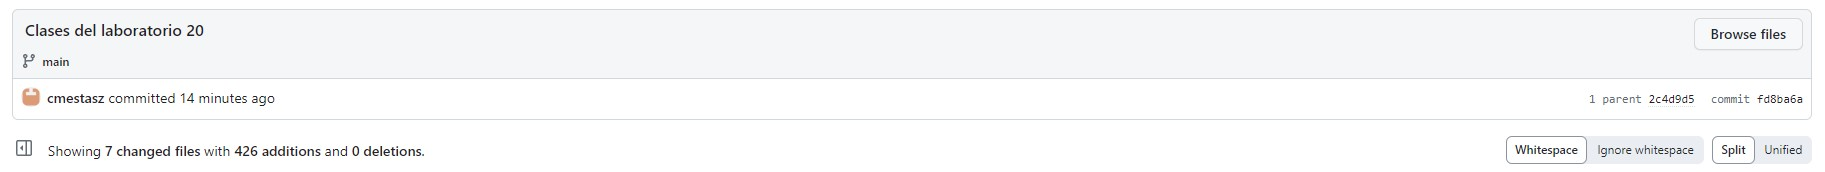
\includegraphics[width=1\textwidth,keepaspectratio]{img/commit01.jpg}
	\caption{Primer Commit.}
\end{figure}
\begin{figure}[H]
	\centering
	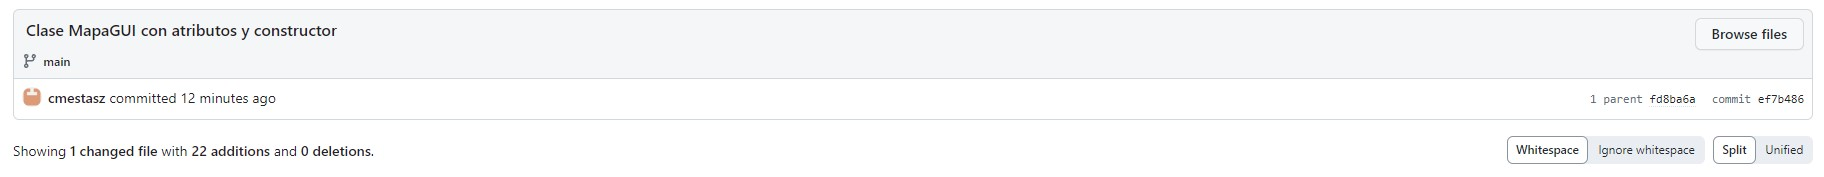
\includegraphics[width=1\textwidth,keepaspectratio]{img/commit02.jpg}
	\caption{Segundo Commit.}
\end{figure}
\begin{figure}[H]
	\centering
	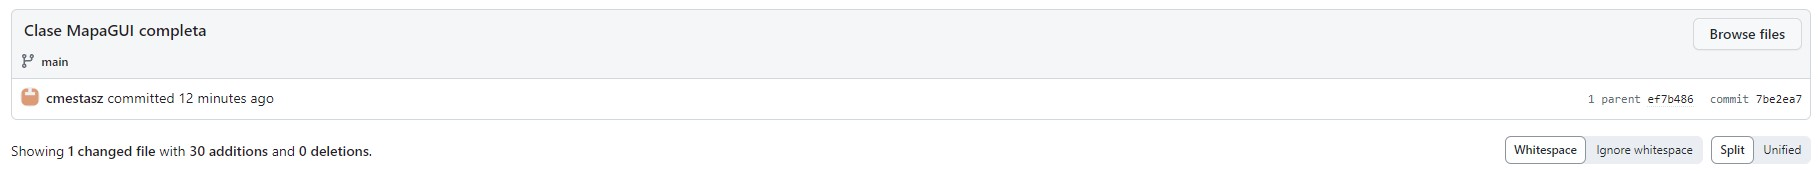
\includegraphics[width=1\textwidth,keepaspectratio]{img/commit03.jpg}
	\caption{Tercer Commit.}
\end{figure}
\begin{figure}[H]
	\centering
	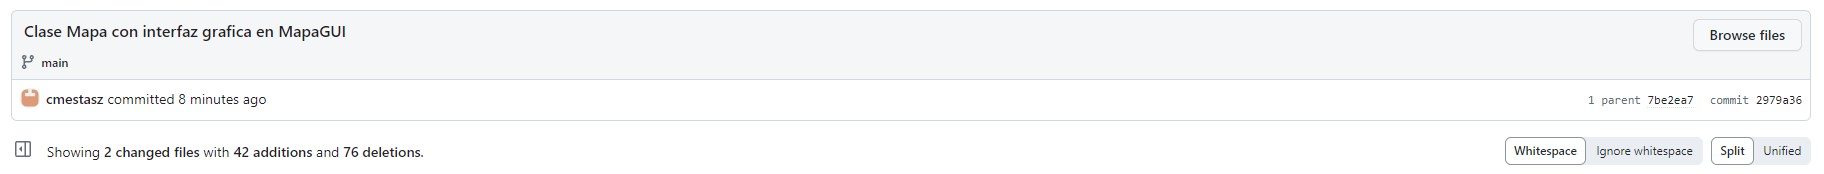
\includegraphics[width=1\textwidth,keepaspectratio]{img/commit04.jpg}
	\caption{Cuarto Commit.}
\end{figure}
\begin{figure}[H]
	\centering
	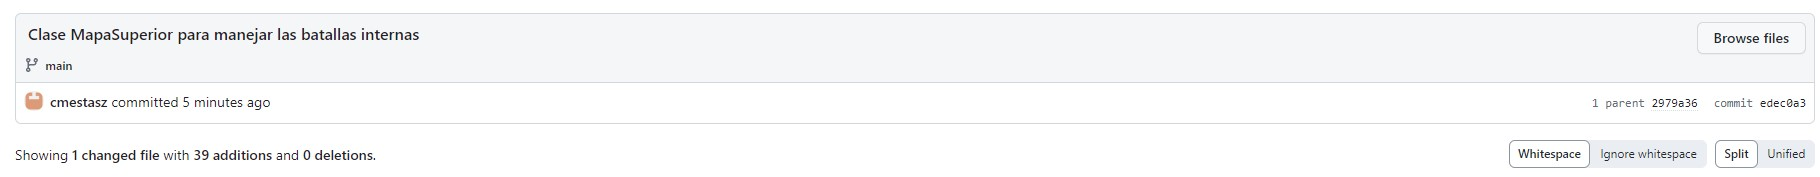
\includegraphics[width=1\textwidth,keepaspectratio]{img/commit05.jpg}
	\caption{Quinto Commit.}
\end{figure}
\begin{figure}[H]
	\centering
	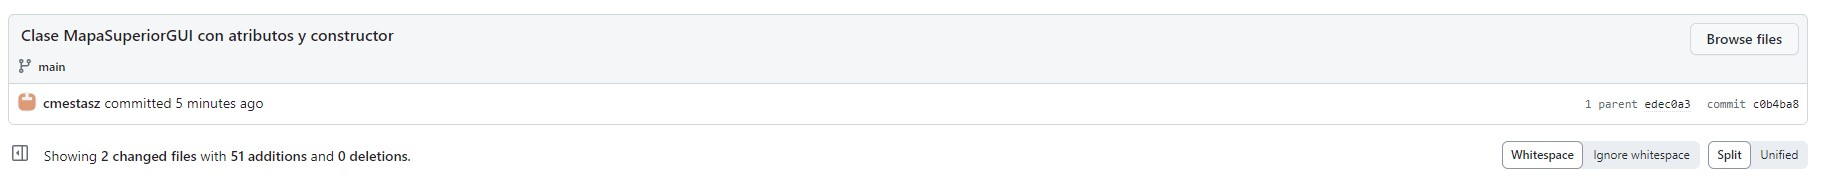
\includegraphics[width=1\textwidth,keepaspectratio]{img/commit06.jpg}
	\caption{Sexto Commit.}
\end{figure}
\begin{figure}[H]
	\centering
	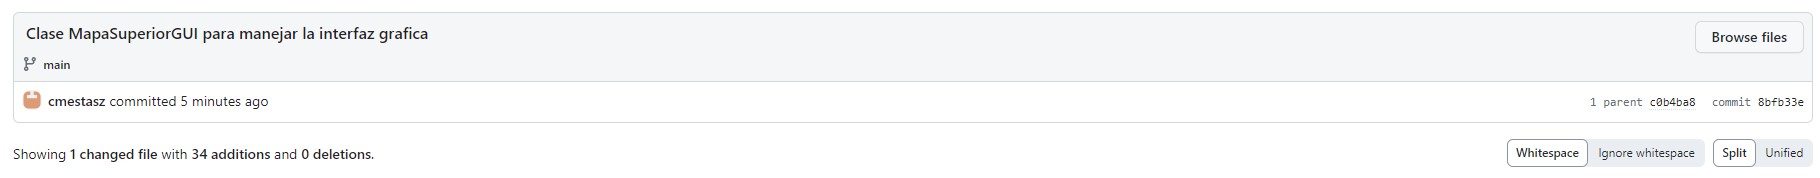
\includegraphics[width=1\textwidth,keepaspectratio]{img/commit07.jpg}
	\caption{Septimo Commit.}
\end{figure}
\begin{figure}[H]
	\centering
	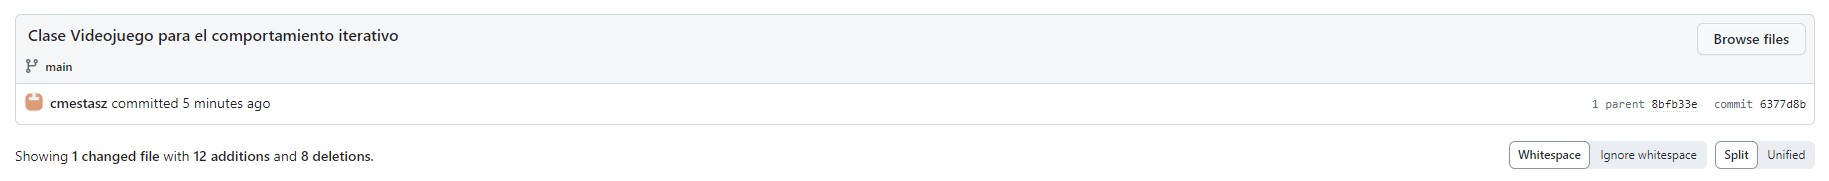
\includegraphics[width=1\textwidth,keepaspectratio]{img/commit08.jpg}
	\caption{Octavo Commit.}
\end{figure}
\pagebreak

\section{Código desarrollado}
\lstinputlisting[language=Java, caption={Soldado.java},numbers=left,]{Soldado.java}
\begin{itemize}
	\item Clase abstracta que guarda nombre y vida del soldado.
	\item Posee getters para todos los atributos.
	\item Posee métodos para el combate como aumentarVida, atacar, herir, defender.
	\item Hereda de la clase JLabel para la interfaz gráfica
\end{itemize}
\lstinputlisting[language=Java, caption={Caballero.java},numbers=left,]{Caballero.java}
\begin{itemize}
	\item Clase que mantiene atributos y métodos independientes de un caballero.
	\item Arma, montado, cambiarArma, montar, desmontar, embestir.
\end{itemize}
\lstinputlisting[language=Java, caption={Arquero.java},numbers=left,]{Arquero.java}
\begin{itemize}
	\item Clase que mantiene atributos y métodos independientes de un arquero.
	\item Flechas, disparar.
\end{itemize}
\lstinputlisting[language=Java, caption={Espadachin.java},numbers=left,]{Espadachin.java}
\begin{itemize}
	\item Clase que mantiene atributos y métodos independientes de un espadachin.
	\item Longitud de espada, generarMuroEscudos.
\end{itemize}
\lstinputlisting[language=Java, caption={Lancero.java},numbers=left,]{Lancero.java}
\begin{itemize}
	\item Clase que mantiene atributos y métodos independientes de un lancero.
	\item Longitud de lanza, schiltrom.
\end{itemize}
\lstinputlisting[language=Java, caption={Mapa.java},numbers=left,]{Mapa.java}
\begin{itemize}
	\item Ciclo de un juego contenido dentro del constructor.
	\item Método inicializarSoldados crea los soldados y los pone en el tablero.
	\item Método verificarVentaja otorga ventaja al reino aventajado por el terreno.
	\item Método obtenerEstado retorna el estado del tablero.
	\item Método obtenerGanador calcula el ganador de la batalla y lo retorna.
	\item Todos los datos se envian a la clase MapaGUI.
\end{itemize}
\lstinputlisting[language=Java, caption={MapaGUI.java},numbers=left,]{MapaGUI.java}
\begin{itemize}
	\item Clase que hereda de JFrame para la interfaz gráfica.
	\item Método mostrarVentana ubica todos los elementos y los muestra
\end{itemize}
\lstinputlisting[language=Java, caption={MapaSuperior.java},numbers=left,]{MapaSuperior.java}
\begin{itemize}
	\item Clase que permite acceder a las diferentes batallas dentro del mapa
	\item Método inicializarBatallas crea las batallas y las pone en el tablero.
	\item Método terminarGuerra regresa el control al juego principal y pregunta al usuario si iniciar otro juego.
\end{itemize}
\lstinputlisting[language=Java, caption={MapaSuperiorGUI.java},numbers=left,]{MapaSuperiorGUI.java}
\begin{itemize}
	\item Clase que hereda de JFrame para la interfaz gráfica.
	\item Método mostrarVentana ubica todos los elementos y los muestra
	\item Se posee la clase interna BotonListener para manejar el evento de acceder a una batalla.
	\item Cuando ya no quedan batallas, la guerra termina.
\end{itemize}
\lstinputlisting[language=Java, caption={Videojuego.java},numbers=left,]{Videojuego.java}
\begin{itemize}
	\item Permite el comportamiento iterativo creando nuevos mapas cada vez que acaba la guerra.
\end{itemize}
\pagebreak

\section{Ejecución del código}
\begin{figure}[H]
	\centering
	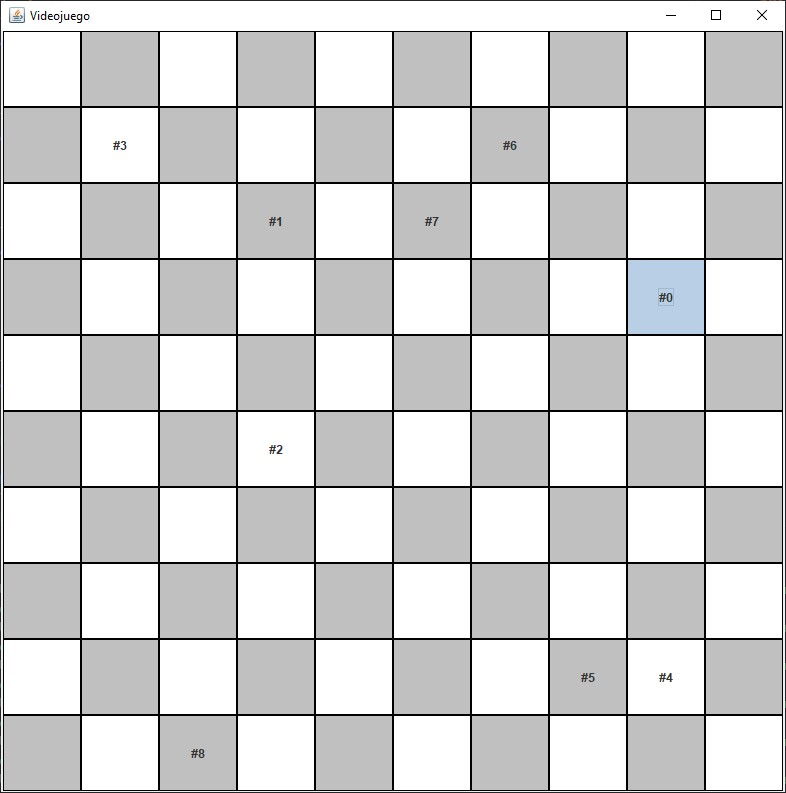
\includegraphics[width=1\textwidth,keepaspectratio]{img/ejec01.jpg}
	\caption{Ejecución.}
\end{figure}
\begin{figure}[H]
	\centering
	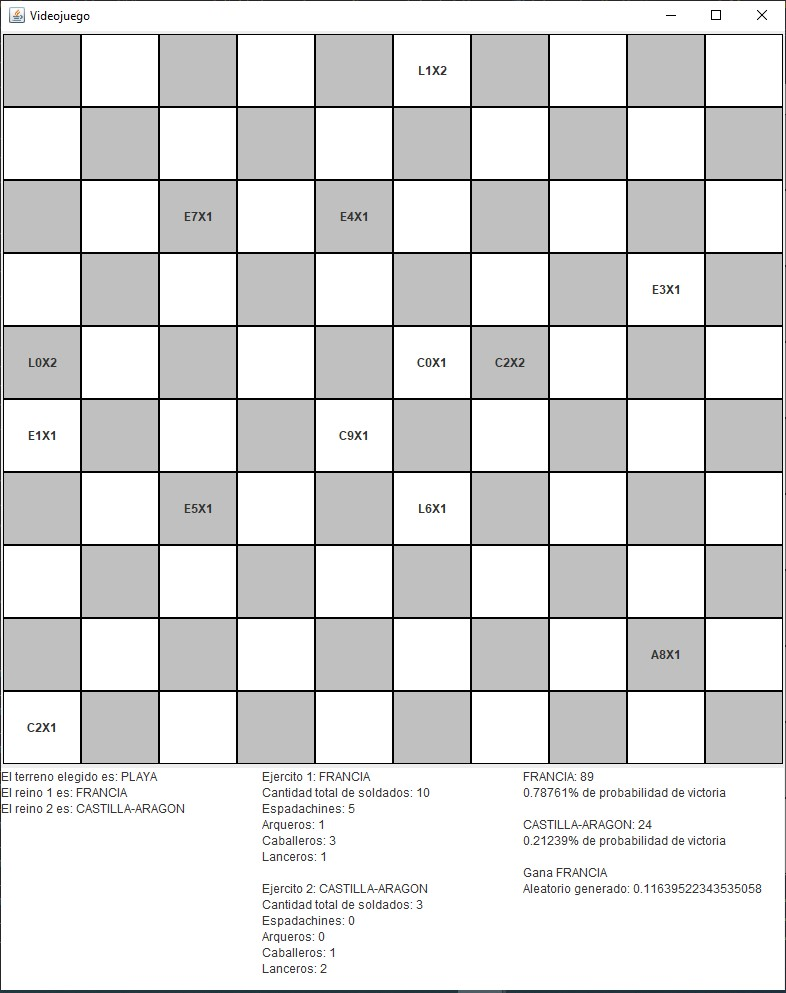
\includegraphics[width=1\textwidth,keepaspectratio]{img/ejec02.jpg}
	\caption{Ejecución.}
\end{figure}
\begin{figure}[H]
	\centering
	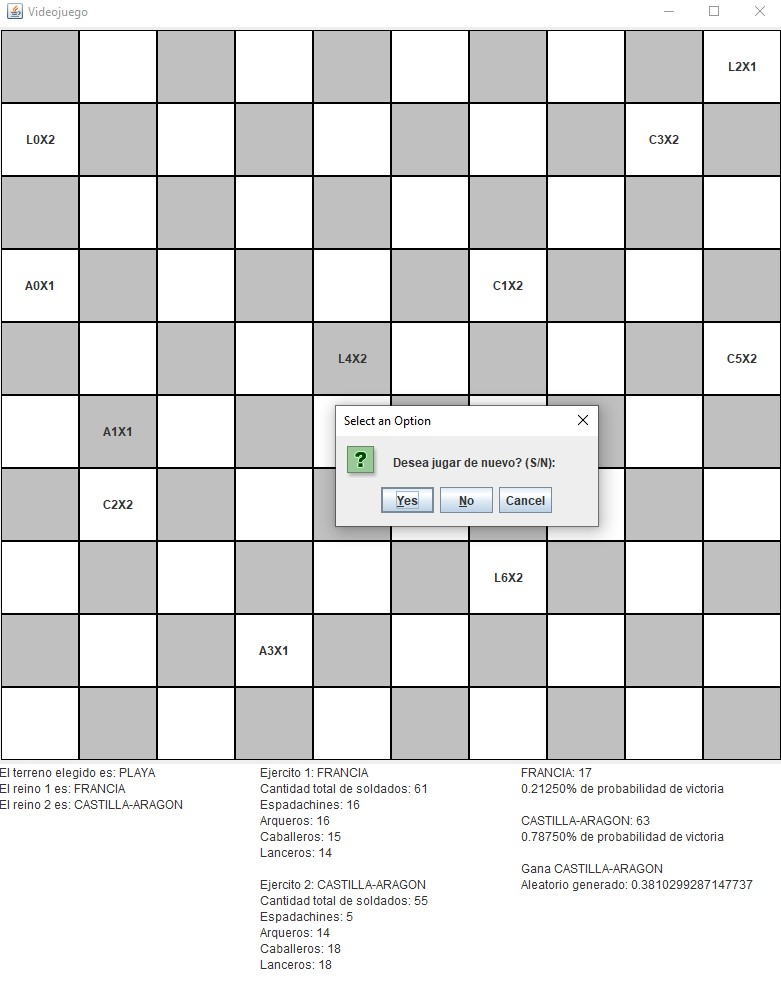
\includegraphics[width=1\textwidth,keepaspectratio]{img/ejec03.jpg}
	\caption{Ejecución.}
\end{figure}
\pagebreak

\section{Diagrama UML}
\begin{figure}[H]
	\centering
	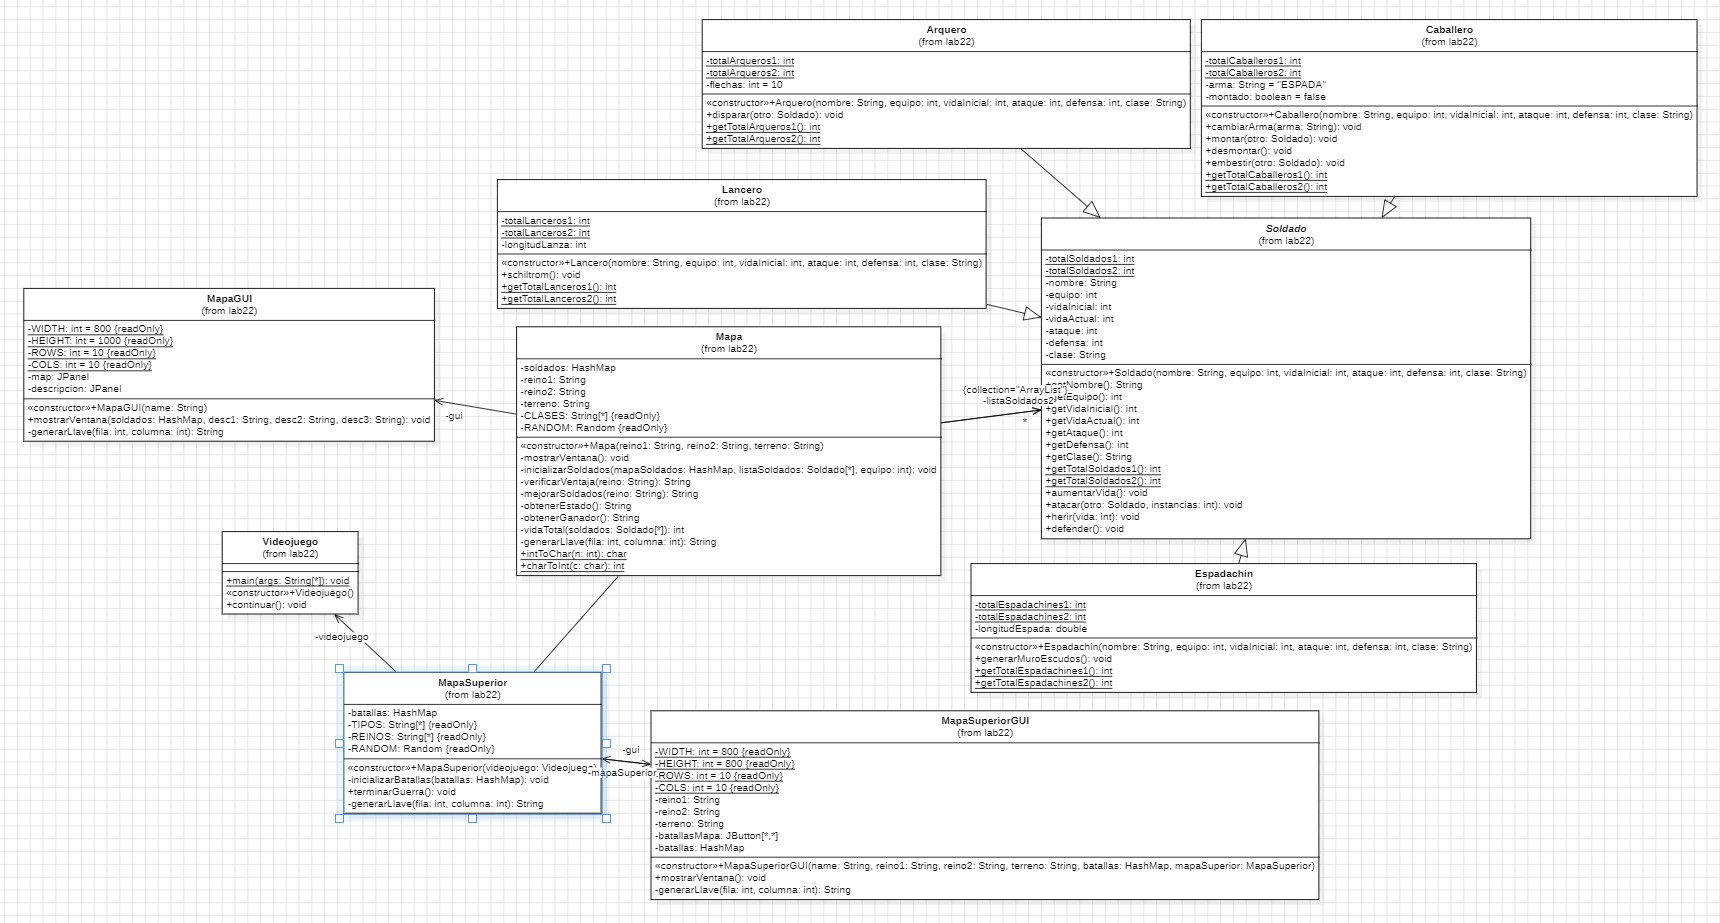
\includegraphics[width=1\textwidth,keepaspectratio]{img/uml.jpg}
	\caption{Diagrama UML.}
\end{figure}
\pagebreak

\section{Estructura de laboratorio \itemPracticeNumber}
\begin{itemize}
	\item El contenido que se entrega en este laboratorio es el siguiente:
\end{itemize}
%%%%%%%%%%%%%%%%%%%%%%%%%%%%%%%%%%%%%%%%%%%%%%%%%%%%%%%%%%%%%%%%%%%%%%
\begin{lstlisting}[style=ascii-tree]
lab22/
|--- Soldado.java
|--- Caballero.java
|--- Arquero.java
|--- Espadachin.java
|--- Lancero.java
|--- Mapa.java
|--- MapaGUI.java
|--- MapaSuperior.java
|--- MapaSuperiorGUI.java
|--- Videojuego.java
|--- commits.bash
|--- Informe.tex
|--- Informe.pdf
|--- img
	|--- logo_abet.png
	|--- logo_episunsa.png
	|--- logo_unsa.jpg
	|--- commit01.jpg
	|--- commit02.jpg
	|--- commit03.jpg
	|--- commit04.jpg
	|--- commit05.jpg
	|--- commit06.jpg
	|--- commit07.jpg
	|--- commit08.jpg
	|--- ejec01.jpg
	|--- ejec02.jpg
	|--- uml.jpg
\end{lstlisting}
%%%%%%%%%%%%%%%%%%%%%%%%%%%%%%%%%%%%%%%%%%%%%%%%%%%%%%%%%%%%%%%%%%%%%%
\pagebreak

\section{\textcolor{red}{Rúbricas}}

\subsection{\textcolor{red}{Entregable Informe}}
\begin{table}[H]
	\caption{Tipo de Informe}
	\setlength{\tabcolsep}{0.5em} % for the horizontal padding
	{\renewcommand{\arraystretch}{1.5}% for the vertical padding
		\begin{tabular}{|M{3cm}|M{12cm}|}
			\hline
			\multicolumn{2}{|c|}{\textbf{\textcolor{red}{Informe}}}                                                                                                      \\
			\hline
			\textbf{\textcolor{red}{Latex}} & \textcolor{blue}{El informe está en formato PDF desde Latex,  con un formato limpio (buena presentación) y facil de leer.} \\
			\hline
		\end{tabular}
	}
\end{table}

\subsection{\textcolor{red}{Rúbrica para el contenido del Informe y demostración}}
\begin{itemize}
	\item El alumno debe marcar o dejar en blanco en celdas de la columna \textbf{Checklist} si cumplio con el ítem correspondiente.
	\item Si un alumno supera la fecha de entrega, su calificación será sobre la nota mínima aprobatoria, siempre y cuando cumpla con todos los items.
	\item El alumno debe autocalificarse en la columna \textbf{Estudiante} de acuerdo a la siguiente tabla:

	      \begin{table}[ht]
		      \caption{Niveles de desempeño}
		      \begin{center}
			      \begin{tabular}{ccccc}
				      \hline
				                      & \multicolumn{4}{c}{Nivel}                                                              \\
				      \cline{1-5}
				      \textbf{Puntos} & Insatisfactorio 25\%      & En Proceso 50\% & Satisfactorio 75\% & Sobresaliente 100\% \\
				      \textbf{2.0}    & 0.5                       & 1.0             & 1.5                & 2.0                 \\
				      \textbf{4.0}    & 1.0                       & 2.0             & 3.0                & 4.0                 \\
				      \hline
			      \end{tabular}
		      \end{center}
	      \end{table}

\end{itemize}

\begin{table}[H]
	\caption{Rúbrica para contenido del Informe y demostración}
	\setlength{\tabcolsep}{0.5em} % for the horizontal padding
	{\renewcommand{\arraystretch}{1.5}% for the vertical padding
		%\begin{center}
		\begin{tabular}{|M{2.3cm}|M{5cm}|M{1.2cm}|M{1.5cm}|M{1.8cm}|M{1.4cm}|}
			\hline
			\multicolumn{2}{|c|}{Contenido y demostración} & Puntos                                                                                                                                                                                                        & Checklist & Estudiante & Profesor   \\
			\hline
			\textbf{1. GitHub}                             & Hay enlace URL activo del directorio para el laboratorio hacia su repositorio GitHub con código fuente terminado y fácil de revisar.                                                                          & 2         & X          & 2        & \\
			\hline
			\textbf{2. Commits}                            & Hay capturas de pantalla de los commits más importantes con sus explicaciones detalladas. (El profesor puede preguntar para refrendar calificación).                                                          & 4         & X          & 4        & \\
			\hline
			\textbf{3. Código fuente}                      & Hay porciones de código fuente importantes con numeración y explicaciones detalladas de sus funciones.                                                                                                        & 2         & X          & 1.5      & \\
			\hline
			\textbf{4. Ejecución}                          & Se incluyen ejecuciones/pruebas del código fuente explicadas gradualmente.                                                                                                                                    & 2         & X          & 1.5      & \\
			\hline
			\textbf{5. Pregunta}                           & Se responde con completitud a la pregunta formulada en la tarea. (El profesor puede preguntar para refrendar calificación).                                                                                   & 2         & X          & 2        & \\
			\hline
			\textbf{6. Fechas}                             & Las fechas de modificación del código fuente estan dentro de los plazos de fecha de entrega establecidos.                                                                                                     & 2         & X          & 2        & \\
			\hline
			\textbf{7. Ortografía}                         & El documento no muestra errores ortográficos.                                                                                                                                                                 & 2         & X          & 1.5      & \\
			\hline
			\textbf{8. Madurez}                            & El Informe muestra de manera general una evolución de la madurez del código fuente,  explicaciones puntuales pero precisas y un acabado impecable. (El profesor puede preguntar para refrendar calificación). & 4         & X          & 4        & \\
			\hline
			\multicolumn{2}{|c|}{\textbf{Total}}           & 20                                                                                                                                                                                                            &           & 18.5       &            \\
			\hline
		\end{tabular}
		%\end{center}
		%\label{tab:multicol}
	}
\end{table}

\section{Referencias}
\begin{itemize}
	\item Aedo, M. y Castro, E. (2021). FUNDAMENTOS DE PROGRAMACIÓN 2 - Tópicos de Programación Orientada a Objetos. Editorial UNSA.
\end{itemize}

%\pagebreak
%\bibliographystyle{apalike}
%\bibliographystyle{IEEEtranN}
%\bibliography{bibliography}

\end{document}